\documentclass[tikz,border=10pt]{standalone}
\usetikzlibrary{decorations.pathreplacing,calc}
\begin{document}
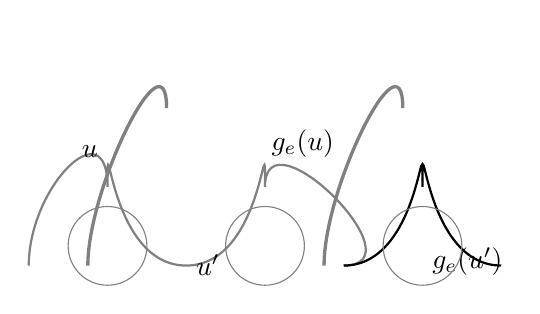
\begin{tikzpicture}[decoration={brace,amplitude=5pt}]
  \draw[gray,thick] (0,0) .. controls ++(90:1) and ++(90:1) .. (1,1) .. controls ++(90:1) and ++(180:1) .. (2,0) .. controls ++(0:1) and ++(90:1) .. (3,1) .. controls ++(90:1) and ++(0:1) .. (4,0);
  \draw[black,thick] (4,0) .. controls ++(0:1) and ++(90:1) .. (5,1) .. controls ++(90:1) and ++(180:1) .. (6,0);
  
  \node[above right] at (2,-0.25) {$u'$};
  \node[above right] at (5,-0.25) {$g_e(u')$};
  \node[above left]  at (1,1.25) {$u$};
  \node[above left]  at (4,1.25) {$g_e(u)$};

  \foreach \i in {1,3,5}
  \draw[gray] (\i,0.25) circle (0.5);
  \draw[very thick, gray] (0.75,0) .. controls ++(90:1) and ++(90:1) .. (1.75,2);
  \draw[very thick, gray] (3.75,0) .. controls ++(90:1) and ++(90:1) .. (4.75,2);
\end{tikzpicture}
\end{document}